\documentclass[]{book}
\usepackage{lmodern}
\usepackage{amssymb,amsmath}
\usepackage{ifxetex,ifluatex}
\usepackage{fixltx2e} % provides \textsubscript
\ifnum 0\ifxetex 1\fi\ifluatex 1\fi=0 % if pdftex
  \usepackage[T1]{fontenc}
  \usepackage[utf8]{inputenc}
\else % if luatex or xelatex
  \ifxetex
    \usepackage{mathspec}
  \else
    \usepackage{fontspec}
  \fi
  \defaultfontfeatures{Ligatures=TeX,Scale=MatchLowercase}
\fi
% use upquote if available, for straight quotes in verbatim environments
\IfFileExists{upquote.sty}{\usepackage{upquote}}{}
% use microtype if available
\IfFileExists{microtype.sty}{%
\usepackage{microtype}
\UseMicrotypeSet[protrusion]{basicmath} % disable protrusion for tt fonts
}{}
\usepackage[margin=1in]{geometry}
\usepackage{hyperref}
\hypersetup{unicode=true,
            pdftitle={Ciencia de Datos y Políticas Públicas},
            pdfauthor={Antonio Vazquez Brust},
            pdfborder={0 0 0},
            breaklinks=true}
\urlstyle{same}  % don't use monospace font for urls
\usepackage{natbib}
\bibliographystyle{apalike}
\usepackage{color}
\usepackage{fancyvrb}
\newcommand{\VerbBar}{|}
\newcommand{\VERB}{\Verb[commandchars=\\\{\}]}
\DefineVerbatimEnvironment{Highlighting}{Verbatim}{commandchars=\\\{\}}
% Add ',fontsize=\small' for more characters per line
\usepackage{framed}
\definecolor{shadecolor}{RGB}{248,248,248}
\newenvironment{Shaded}{\begin{snugshade}}{\end{snugshade}}
\newcommand{\KeywordTok}[1]{\textcolor[rgb]{0.13,0.29,0.53}{\textbf{#1}}}
\newcommand{\DataTypeTok}[1]{\textcolor[rgb]{0.13,0.29,0.53}{#1}}
\newcommand{\DecValTok}[1]{\textcolor[rgb]{0.00,0.00,0.81}{#1}}
\newcommand{\BaseNTok}[1]{\textcolor[rgb]{0.00,0.00,0.81}{#1}}
\newcommand{\FloatTok}[1]{\textcolor[rgb]{0.00,0.00,0.81}{#1}}
\newcommand{\ConstantTok}[1]{\textcolor[rgb]{0.00,0.00,0.00}{#1}}
\newcommand{\CharTok}[1]{\textcolor[rgb]{0.31,0.60,0.02}{#1}}
\newcommand{\SpecialCharTok}[1]{\textcolor[rgb]{0.00,0.00,0.00}{#1}}
\newcommand{\StringTok}[1]{\textcolor[rgb]{0.31,0.60,0.02}{#1}}
\newcommand{\VerbatimStringTok}[1]{\textcolor[rgb]{0.31,0.60,0.02}{#1}}
\newcommand{\SpecialStringTok}[1]{\textcolor[rgb]{0.31,0.60,0.02}{#1}}
\newcommand{\ImportTok}[1]{#1}
\newcommand{\CommentTok}[1]{\textcolor[rgb]{0.56,0.35,0.01}{\textit{#1}}}
\newcommand{\DocumentationTok}[1]{\textcolor[rgb]{0.56,0.35,0.01}{\textbf{\textit{#1}}}}
\newcommand{\AnnotationTok}[1]{\textcolor[rgb]{0.56,0.35,0.01}{\textbf{\textit{#1}}}}
\newcommand{\CommentVarTok}[1]{\textcolor[rgb]{0.56,0.35,0.01}{\textbf{\textit{#1}}}}
\newcommand{\OtherTok}[1]{\textcolor[rgb]{0.56,0.35,0.01}{#1}}
\newcommand{\FunctionTok}[1]{\textcolor[rgb]{0.00,0.00,0.00}{#1}}
\newcommand{\VariableTok}[1]{\textcolor[rgb]{0.00,0.00,0.00}{#1}}
\newcommand{\ControlFlowTok}[1]{\textcolor[rgb]{0.13,0.29,0.53}{\textbf{#1}}}
\newcommand{\OperatorTok}[1]{\textcolor[rgb]{0.81,0.36,0.00}{\textbf{#1}}}
\newcommand{\BuiltInTok}[1]{#1}
\newcommand{\ExtensionTok}[1]{#1}
\newcommand{\PreprocessorTok}[1]{\textcolor[rgb]{0.56,0.35,0.01}{\textit{#1}}}
\newcommand{\AttributeTok}[1]{\textcolor[rgb]{0.77,0.63,0.00}{#1}}
\newcommand{\RegionMarkerTok}[1]{#1}
\newcommand{\InformationTok}[1]{\textcolor[rgb]{0.56,0.35,0.01}{\textbf{\textit{#1}}}}
\newcommand{\WarningTok}[1]{\textcolor[rgb]{0.56,0.35,0.01}{\textbf{\textit{#1}}}}
\newcommand{\AlertTok}[1]{\textcolor[rgb]{0.94,0.16,0.16}{#1}}
\newcommand{\ErrorTok}[1]{\textcolor[rgb]{0.64,0.00,0.00}{\textbf{#1}}}
\newcommand{\NormalTok}[1]{#1}
\usepackage{longtable,booktabs}
\usepackage{graphicx,grffile}
\makeatletter
\def\maxwidth{\ifdim\Gin@nat@width>\linewidth\linewidth\else\Gin@nat@width\fi}
\def\maxheight{\ifdim\Gin@nat@height>\textheight\textheight\else\Gin@nat@height\fi}
\makeatother
% Scale images if necessary, so that they will not overflow the page
% margins by default, and it is still possible to overwrite the defaults
% using explicit options in \includegraphics[width, height, ...]{}
\setkeys{Gin}{width=\maxwidth,height=\maxheight,keepaspectratio}
\IfFileExists{parskip.sty}{%
\usepackage{parskip}
}{% else
\setlength{\parindent}{0pt}
\setlength{\parskip}{6pt plus 2pt minus 1pt}
}
\setlength{\emergencystretch}{3em}  % prevent overfull lines
\providecommand{\tightlist}{%
  \setlength{\itemsep}{0pt}\setlength{\parskip}{0pt}}
\setcounter{secnumdepth}{5}
% Redefines (sub)paragraphs to behave more like sections
\ifx\paragraph\undefined\else
\let\oldparagraph\paragraph
\renewcommand{\paragraph}[1]{\oldparagraph{#1}\mbox{}}
\fi
\ifx\subparagraph\undefined\else
\let\oldsubparagraph\subparagraph
\renewcommand{\subparagraph}[1]{\oldsubparagraph{#1}\mbox{}}
\fi

%%% Use protect on footnotes to avoid problems with footnotes in titles
\let\rmarkdownfootnote\footnote%
\def\footnote{\protect\rmarkdownfootnote}

%%% Change title format to be more compact
\usepackage{titling}

% Create subtitle command for use in maketitle
\newcommand{\subtitle}[1]{
  \posttitle{
    \begin{center}\large#1\end{center}
    }
}

\setlength{\droptitle}{-2em}

  \title{Ciencia de Datos y Políticas Públicas}
    \pretitle{\vspace{\droptitle}\centering\huge}
  \posttitle{\par}
  \subtitle{Una introducción a la exploración, análisis y visualización de datos}
  \author{Antonio Vazquez Brust}
    \preauthor{\centering\large\emph}
  \postauthor{\par}
      \predate{\centering\large\emph}
  \postdate{\par}
    \date{2019-03-24}

\usepackage{booktabs}

\begin{document}
\maketitle

{
\setcounter{tocdepth}{1}
\tableofcontents
}
\chapter*{}\label{section}
\addcontentsline{toc}{chapter}{}

Placeholder

\section*{Antes de empezar}\label{antes-de-empezar}
\addcontentsline{toc}{section}{Antes de empezar}

\chapter{¿Qué es la ciencia de datos?}\label{que-es-la-ciencia-de-datos}

Placeholder

\section{¿Qué significa hacer ciencia de
datos?}\label{que-significa-hacer-ciencia-de-datos}

\chapter{Una presentación a toda marcha de
R}\label{una-presentacion-a-toda-marcha-de-r}

\texttt{R} es un lenguaje de programación especializado en análisis y
visualización de datos. Es un producto de código abierto, lo cual
significa que cualquier persona puede usarlo y modificarlo sin pagar
licencias ni costos de adquisición de ningún tipo.

Expertos de todo el mundo colaboran en forma activa con el proyecto, no
sólo desarrollando el lenguaje en sí (llamado ``R base''), sino también
extendiéndolo con nuevas habilidades que pueden ser incorporadas por los
usuarios finales en forma de ``paquetes'' instalables.

La calidad del lenguaje en sí, de los paquetes instalables que le
agregan un sinfín de funciones (desde algoritmos de inteligencia
artificial hasta mapas interactivos) y de la comunidad de usuarios que
comparte información en foros y blogs, ha hecho de R uno de los
lenguajes de programación más populares del mundo. En el campo del
análisis de datos, es la herramienta por excelencia en muchas
universidades, empresas de tecnología, y redacciones de periodismo de
datos.

\section{Nuestro primer proyecto en
R}\label{nuestro-primer-proyecto-en-r}

A continuación reproduciremos un ejercicio paso a paso, para ilustrar la
potencia de una herramienta de análisis como R. Que nadie se preocupe si
algunas de las operaciones parecen no tener sentido, o resultan
arbitrarias. ¡Es normal! Nadie aprende un lenguaje en 10 minutos, sea R
o esperanto. La idea es tener exposición temprana a un caso de uso
interesante, usando datos reales. Y que nos sirva como motivación para
practicar luego ejercicios básicos que son muy necesarios pero, a veces,
no tan emocionantes.

\subsection{Crear un proyecto en
RStudio}\label{crear-un-proyecto-en-rstudio}

El primer paso es ejecutar RStudio, que ya deberíamos tener disponible
en nuestro sistema.

Una vez abierta la interfaz gráfica, creamos un proyecto nuevo,
cliqueando en
\texttt{File\ -\textgreater{}\ New\ Project...\ -\textgreater{}\ New\ Directory\ -\textgreater{}\ \ New\ Project}.
En la ventana que surge, elegir un nombre para el proyecto (por ejemplo,
``Practicando R'') y finalizar la operación cliqueando en
\texttt{Create\ project}.

Utilizar proyectos nos permite continuar otro día desde donde dejamos la
tarea al terminar una sesión. Es sólo cuestión de recuperar el proyecto
deseado la próxima vez que abrimos RStudio, cliqueando en
\texttt{File\ -\textgreater{}\ Recent\ Projects\ -\textgreater{}\ "nombre\ de\ mi\ proyecto"}.

Por ahora, sigamos trabajando. Vamos a crear un ``script''. Un script,
como su nombre en inglés lo indica, es un guión; una serie de pasos que
escribimos para que nuestra computadora ejecute en secuencia. Cliqueamos
en
\texttt{File\ -\textgreater{}\ New\ File\ -\textgreater{}\ R\ Script}.
De inmediato se abre una ventana con un editor de texto. ¡Ahora empieza
la acción!

\subsection{Escribiendo un script}\label{escribiendo-un-script}

Aprovechemos para dar un nombre a los áreas que vemos en RStudio:

\begin{figure}
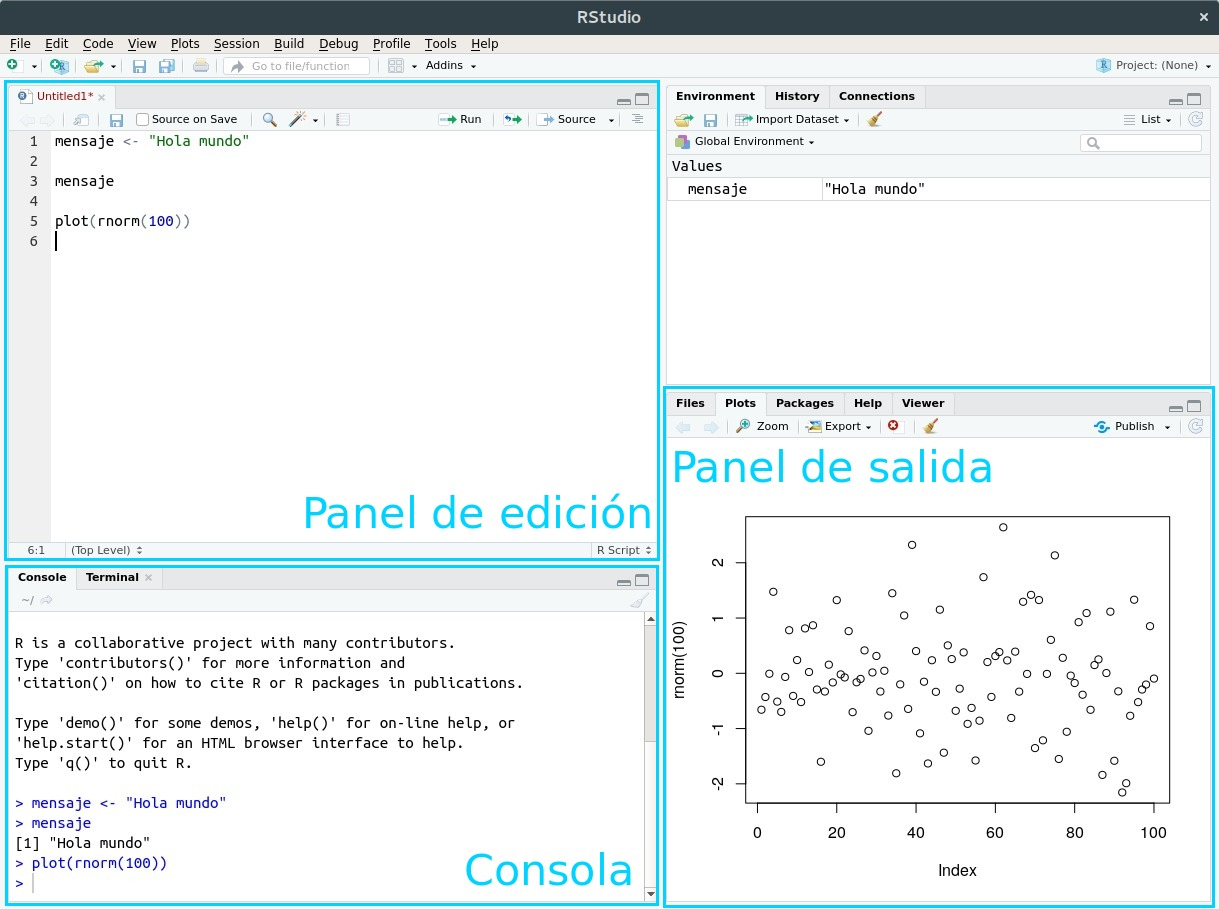
\includegraphics[width=1\linewidth]{imagenes/Interfaz_RStudio} \caption{La interfaz de RStudio}\label{fig:unnamed-chunk-1}
\end{figure}

Vamos a escribir nuestro código (las instrucciones que \texttt{R}
entiende) en el panel de edición. Los resultados van a aparecer en la
consola (cuando se trate de texto) o en el panel de salida (cuando
produzcamos gráficos)

Por ejemplo, podemos escribir el panel de edición la instrucción para
mostrar el resultado de una operación matemático:

\begin{Shaded}
\begin{Highlighting}[]
\KeywordTok{sqrt}\NormalTok{(}\DecValTok{144}\NormalTok{)}
\end{Highlighting}
\end{Shaded}

\texttt{sqrt()} es una \emph{función}. En el mundo de la programación,
las funciones son secuencias de código ya listas para usar, que realizan
tareas útiles. Por ejemplo, mostrar algo en pantalla. En nuestro caso,
completamos la función con algo más: un \emph{parámetro}, pues así se le
llama a los valores que una función espera de parte del usuario para
saber que hacer. La función print espera que le demos un número para el
cual calcular su raíz cuadrada (\emph{square root} en inglés), y eso
hicimos: le pasamos cómo parámetro \texttt{144}, un número. Los
parámetros siempre se escriben entre paréntesis, a continuación del
nombre de la función.

Ahora vamos a aprender la combinación de teclas más importante al usar
RStudio: \texttt{Ctrl} + \texttt{Enter}. Presionar \texttt{Ctrl} +
\texttt{Enter} al terminar de escribir una instrucción hace que RStudio
la ejecute de inmediato, y espere en la siguiente instrucción, si la
hubiera.

Cambien podemos buscar una línea que deseemos ejecutar, posicionando el
cursor de texto (que luce como una barra vertical que titila, en el
panel de edición) sobre ella. Si a continuación pulsamos \texttt{Ctrl} +
\texttt{Enter}, la línea será ejecutada y el cursor se moverá sólo hasta
la siguiente línea, listo para repetir el proceso.

La modalidad de ejecución línea por línea es muy útil para lo que se
llama ``análisis interactivo''. Uno ejecuta un comando, observa el
resultado, y en base a eso decide su próxima acción: cambiar parámetros
e intentarlo de nuevo, dar por buenos los resultados y usarlos para una
tarea subsiguiente\ldots{} etc.

Por ejemplo, si escribimos las siguientes líneas:

\begin{Shaded}
\begin{Highlighting}[]
\KeywordTok{sqrt}\NormalTok{(}\DecValTok{144}\NormalTok{)}

\NormalTok{mensaje <-}\StringTok{ "Hola mundo"}

\NormalTok{mensaje}
\end{Highlighting}
\end{Shaded}

\ldots{}y posicionamos el cursor en cualquier posición de la primera
línea, para luego pulsar \texttt{Ctrl} + \texttt{Enter} tres veces,
veremos que las instrucciones son ejecutadas línea a línea.

\begin{Shaded}
\begin{Highlighting}[]
\KeywordTok{sqrt}\NormalTok{(}\DecValTok{144}\NormalTok{)}
\end{Highlighting}
\end{Shaded}

\begin{verbatim}
## [1] 12
\end{verbatim}

\begin{Shaded}
\begin{Highlighting}[]
\NormalTok{mensaje <-}\StringTok{ "Hola mundo"}
\end{Highlighting}
\end{Shaded}

\begin{Shaded}
\begin{Highlighting}[]
\NormalTok{mensaje}
\end{Highlighting}
\end{Shaded}

\begin{verbatim}
## [1] "Hola mundo"
\end{verbatim}

Dos de ellas (la primera y la última) mostraron una salida en pantalla,
y la del medio, no. Esto es porque algunas funciones entregan algo como
resultado algo -un número, un texto, un gráfico, u otros tipos de salida
que ya veremos- mientras que otras hacen su tarea silenciosamente sin
expresar nada. En este caso, la función silenciosa fue la de asignación:
\texttt{mensaje\ \textless{}-\ "Hola\ mundo"} es una instrucción que le
pide a R que cree una variable llamada ``mensaje'' (o que la encuentre
si ya existe) y que le asigne como valor el texto ``Hola mundo''. ¿Cómo
sabemos que la instrucción se llevó a cabo, a pesar de no producir una
salida? En general, es un tema de confianza. Si una instrucción no
genera un mensaje de error, si es silenciosa, se asume que pudo cumplir
su cometido. En este caso, además lo hemos verificado. La línea final,
\texttt{mensaje} pide a R que busque la variable, y muestre en pantalla
su contenido (esa es una característica muy práctica del lenguaje: para
saber el contenido de una variable, basta con escribirla y ejecutar la
línea). Y al hacerlo, comprobamos que la variable contiene precisamente
lo que hemos tipeado.

De paso, hay que mencionar que la creación y manipulación de variables
es un concepto clave en programación. Trabajar con variables nos permite
almacenar valores para usarlos después, además de hacer nuestro código
más fácil de leer y compartir con otros, en especial cuando usamos
nombre de variable auto-explicativos. Como ejemplo de ésto ultimo
comparemos

\begin{Shaded}
\begin{Highlighting}[]
\NormalTok{x <-}\StringTok{ }\DecValTok{8} \OperatorTok{*}\StringTok{ }\DecValTok{6}
\NormalTok{x}
\end{Highlighting}
\end{Shaded}

\begin{verbatim}
## [1] 48
\end{verbatim}

\ldots{} con

\begin{Shaded}
\begin{Highlighting}[]
\NormalTok{ancho_habitacion_m <-}\StringTok{ }\DecValTok{8}
\NormalTok{profundiad_habitacion_m <-}\StringTok{ }\DecValTok{6}
\NormalTok{superficie_habitacion_m2 <-}\StringTok{ }\NormalTok{ancho_habitacion_m }\OperatorTok{*}\StringTok{ }\NormalTok{profundiad_habitacion_m}

\NormalTok{superficie_habitacion_m2}
\end{Highlighting}
\end{Shaded}

\begin{verbatim}
## [1] 48
\end{verbatim}

En su resultado ambas expresiones son iguales, dado que producen lo
mismo. Pero la segunda esta escrita de una forma mucho más clara para un
ser humano, que hace más fácil interpretar su lógica\ldots{} ¡está
calculando la superficie en metros cuadrados de una habitación!. Es muy
importante escribir nuestro código de la forma más explícita posible,
aunque requiera tipear un poco más. Con ello, le hacemos la vida más
fácil a otras personas que interpreten nuestros programas. Y también a
nosotros mismos en el futuro, cuando debamos lidiar con un programa que
escribimos tiempo atrás y del que a duras penas recordamos su lógica.

\section{Un ejemplo de análisis paso a
paso}\label{un-ejemplo-de-analisis-paso-a-paso}

\includegraphics{https://media.giphy.com/media/fVeAI9dyD5ssIFyOyM/giphy.gif}
\textless{}\textless{}\textless{} \ldots{}en construcción\ldots{}
\textgreater{}\textgreater{}\textgreater{}

\begin{verbatim}
## Linking to GEOS 3.6.2, GDAL 2.2.3, PROJ 4.9.3
\end{verbatim}

En los siguientes capítulos practicaremos varias técnicas que nos
permitirán profundizar nuestros análisis, en la nunca finalizada misión
de entender un poco más.

\chapter{Poniendo los datos en forma}\label{poniendo-los-datos-en-forma}

Placeholder

\section{Primeros pasos al examinar un conjunto de datos
nuevo}\label{primeros-pasos-al-examinar-un-conjunto-de-datos-nuevo}

\section{\texorpdfstring{Cruzando variables: la operación
\texttt{join}}{Cruzando variables: la operación join}}\label{cruzando-variables-la-operacion-join}

\section{Transformando los datos}\label{transformando-los-datos}

\subsection{\texorpdfstring{Seleccionar columnas con
\texttt{select()}}{Seleccionar columnas con select()}}\label{seleccionar-columnas-con-select}

\subsection{\texorpdfstring{Filtrar filas con
\texttt{filter()}}{Filtrar filas con filter()}}\label{filtrar-filas-con-filter}

\subsubsection{Comparaciones}\label{comparaciones}

\subsubsection{Operadores lógicos}\label{operadores-logicos}

\subsection{\texorpdfstring{Ordenar filas con
\texttt{arrange()}}{Ordenar filas con arrange()}}\label{ordenar-filas-con-arrange}

\subsubsection{Valores faltantes}\label{valores-faltantes}

\subsection{\texorpdfstring{Agregar nuevas variables con
\texttt{mutate()}}{Agregar nuevas variables con mutate()}}\label{agregar-nuevas-variables-con-mutate}

\subsection{\texorpdfstring{Extraer sumarios con
\texttt{summarise()}}{Extraer sumarios con summarise()}}\label{extraer-sumarios-con-summarise}

\subsection{\texorpdfstring{¡BONUS! El operador ``pipe'':
\texttt{\%\textgreater{}\%}}{¡BONUS! El operador pipe: \%\textgreater{}\%}}\label{bonus-el-operador-pipe}

\chapter{Visualización}\label{visualizacion}

Placeholder

\section{\texorpdfstring{Una buena visualización para empezar: el
\emph{scatterplot}}{Una buena visualización para empezar: el scatterplot}}\label{una-buena-visualizacion-para-empezar-el-scatterplot}

\section{Ajustando color y tamaño}\label{ajustando-color-y-tamano}

\section{Facetado}\label{facetado}

\section{Gráficos de barras}\label{graficos-de-barras}

\section{Histogramas}\label{histogramas}

\section{Preparando una visualización para
compartir}\label{preparando-una-visualizacion-para-compartir}

\section{Otras visualizaciones}\label{otras-visualizaciones}

\chapter{Modelado estadístico}\label{modelado-estadistico}

Placeholder

\section{Regresión lineal simple}\label{regresion-lineal-simple}

\subsection{Regresión con una variable
numérica}\label{regresion-con-una-variable-numerica}

\subsection{Revolviendo los residuos}\label{revolviendo-los-residuos}

\subsection{Regresión con una variable
categórica}\label{regresion-con-una-variable-categorica}

\section{Regresión con múltiples
variables}\label{regresion-con-multiples-variables}

\chapter{Información geográfica y
mapas}\label{informacion-geografica-y-mapas}

Placeholder

\section{Los datos georreferenciados}\label{los-datos-georreferenciados}

\section{Formatos de archivo}\label{formatos-de-archivo}

\section{Explorando un archivo con información
geográfica}\label{explorando-un-archivo-con-informacion-geografica}

\section{Visualizando información
geográfica}\label{visualizando-informacion-geografica}

\section{Volcando en el mapa información de múltiples
fuentes}\label{volcando-en-el-mapa-informacion-de-multiples-fuentes}

\section{Combinando capas
geográficas}\label{combinando-capas-geograficas}

\bibliography{book.bib,packages.bib}


\end{document}
